\documentclass[../main/report.tex]{subfiles}
\begin{document}

\section{Output}
The main source of output from the FPGA is an HDMI connector.
This is a novel feature this year, as no previous group has tried to implement it before.

Because of this new challenge, a lot of backup schemes were put in place.
The HDMI connector is put on headers, in case the connector fails.
A separate VGA module is connected to the FPGA, in case the HDMI doesn't work and if this fails, a VGA module is also connected to the microcontroller.

\subsection{HDMI implementation}

The general HDMI specification consists of the Transition Minimized Differential Signaling(TMDS), and some additional wires for details regarding the transmitted signal ~\cite{hdmi-pinout}.
However, we were able to produce a video feed on a screen from an FPGA using only the TMDS wires by cutting up an HDMI cable and using only those wires.
Upon seeing that this was feasible, we decided to make the HDMI hardware with a TMDS connection only, going in to the FPGA. The resulting hardware was then an HDMI type-A receptacle footprint, the HDMI receptacle and a header between it and the FPGA.
The reason for adding the header was that this setup is equivalent to the aforementioned prototype version so that if the HDMI input wouldn't work we could connect the (header)terminated HDMI cable onto the header.

\begin{figure}[H]
	\centering
	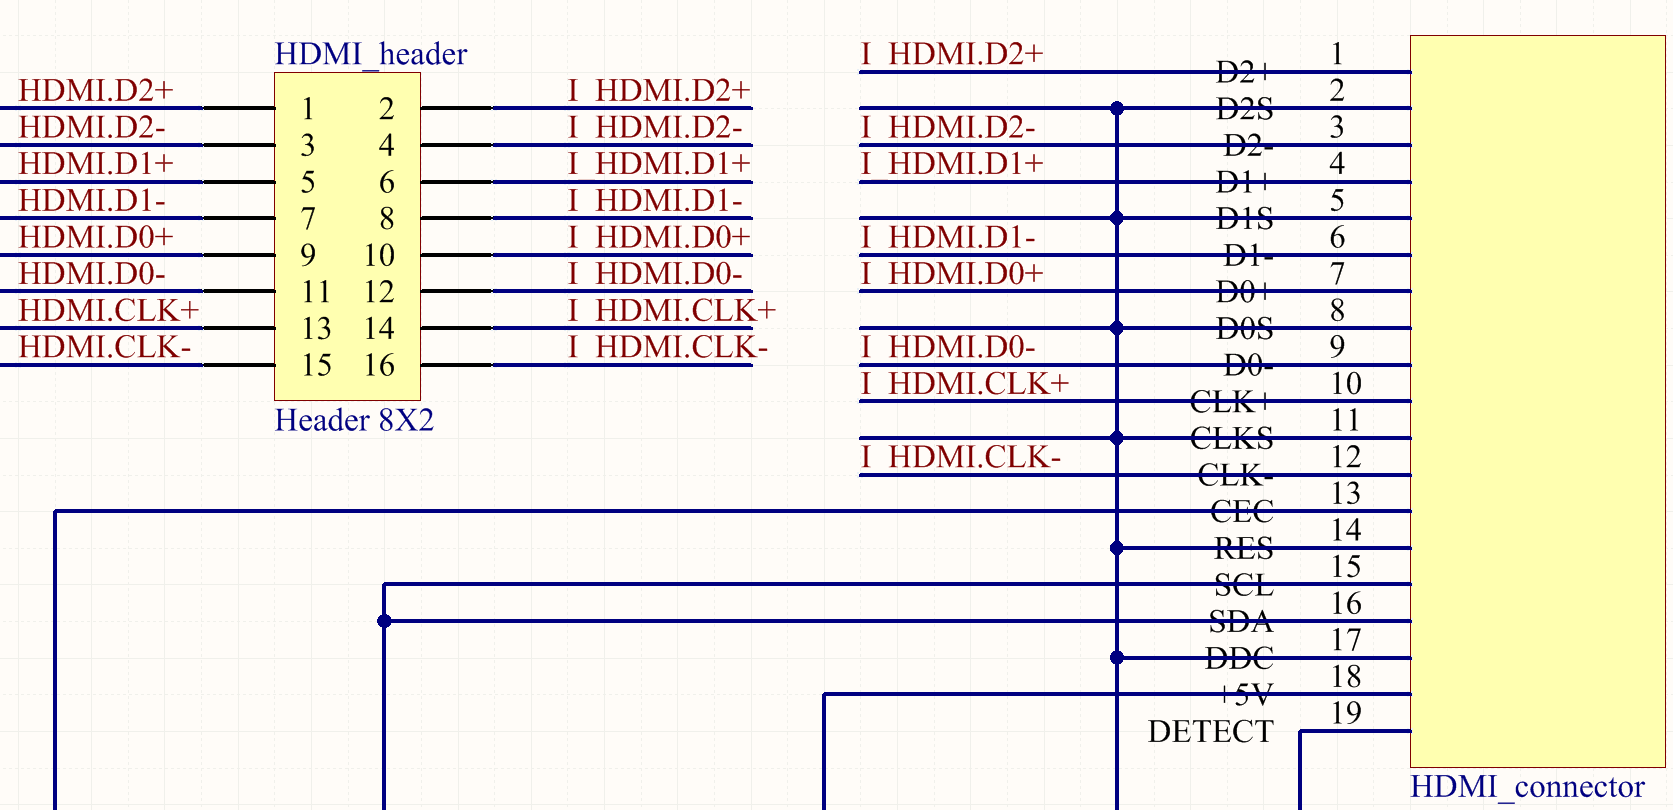
\includegraphics[width=0.85\textwidth]{../pcb/assets/HDMI-schematic.png}
	\caption{Schematic view of the HDMI circuit}
	\label{fig: HDMI schematic}
\end{figure}
\end{document}
